\documentclass{article}
\usepackage[utf8]{inputenc}
\usepackage{multicol}
\usepackage{listings}
\usepackage{amssymb}
\usepackage{enumitem}
\usepackage{graphicx}
\usepackage{amsthm}
\usepackage{hyperref}
\usepackage{tikz}
\usepackage[ruled,vlined]{algorithm2e}
\usepackage{ulem}
\newtheorem{theorem}{Theorem}
\newtheorem{definition}{Definition}
\newcommand{\N}{\mathbb{N}}
\newcommand{\Np}{{\mathbb{N}^{>0}}}
\newcommand{\Z}{\mathbb{Z}}
\newcommand{\R}{\mathbb{R}}
\newcommand{\bigO}{\mathcal{O}}
\newcommand{\code}[1]{\texttt{#1}}
\newcommand{\hints}[1]{\paragraph{\bf Hints:} #1}

\usetikzlibrary{arrows, positioning}

%=====================================
%			Assignment 8
%=====================================

\begin{document}

\title{Weekly Assignment 8}
\date{26th October 2017}
\author{Tony Lopar \\ s1013792}
\maketitle

\paragraph{Deadline:} 15th November 2017, 6pm.
\paragraph{Solutions:} Solutions can be found below the exercises!

\section*{Part I. Red-Black Trees.}




\subsection*{Exercise 1. \textit{Weight: 5\%}}
Given the following RBT:
% \begin{figure}[h!]
% \centering
% \includegraphics[width=12cm]{img/rbt-1.png}
% \end{figure}

\begin{enumerate}
	\item Give $bh(30)$, $bh(20)$, $bh(35)$ and $bh(50)$.
\end{enumerate}

\subsection*{Solutions 1}
\begin{enumerate}
	\item $bh(30) = 3$
	\item $bh(20) = 3$
	\item $bh(35) = 2$
	\item $bh(50) = 1$

\end{enumerate}

\newpage
\subsection*{Exercise 2. \textit{Weight: 15\%}}
Draw the RBT that result after successively inserting $30$, $15$, $10$, $19$, $22$, $50$. Delete $10$ and then $30$. Draw the resulting trees after each operation (\textit{each} insertion and \textit{each} deletion).

 \subsection*{Solutions 2}
 The first step is to insert the red node 30. Since this is the root, we immediately fix the color to black. \\
 \begin{center}
 
\begin{tikzpicture}[-, level/.style={sibling distance = 2cm/#1, level distance = 1.5cm}, scale=1,transform shape]
   \node[circle,draw, fill=black, text=white](z){$30$};
 \end{tikzpicture}
 \end{center}

Then we instert 15. Since it's lower than the root, it will be on the left. The node may remain red, because no properties of a red-black tree are vialoted. \\
\begin{center}
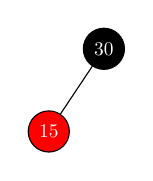
\begin{tikzpicture}[-, level/.style={sibling distance = 2cm/#1, level distance = 1.5cm}, scale=0.7,transform shape]
	\node[circle,draw, fill=black, text=white](z){$30$}
			child{
					node[circle,draw, fill=red, text=white]{15}
			}
			child[missing];
\end{tikzpicture}
\end{center}

Next, we instert 10. This value is lower than 20 and 15, so we place it left below 20. But since the node has a black uncle, we will perform a right rotate and we will recolor 15 to black, because it's the new root. Furthermore, node 30 will be recolored to red as part of the fixup.

\begin{center}
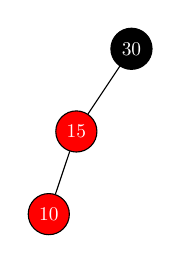
\begin{tikzpicture}[-, level/.style={sibling distance = 2cm/#1, level distance = 1.5cm}, scale=0.7,transform shape]
	\node[circle,draw, fill=black, text=white](z){$30$}
			child{
					node[circle,draw, fill=red, text=white]{15}
					child {
						node[circle,draw, fill=red, text=white]{10}
					}
					child[missing]
			}
			child[missing];
\end{tikzpicture}
$\Rightarrow$
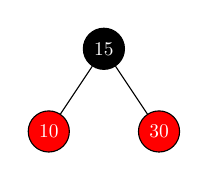
\begin{tikzpicture}[-, level/.style={sibling distance = 2cm/#1, level distance = 1.5cm}, scale=0.7,transform shape]
	\node[circle,draw, fill=black, text=white](z){$15$}
			child{
					node[circle,draw, fill=red, text=white]{10}
			}
			child{
				node[circle,draw, fill=red, text=white]{30}
			};
\end{tikzpicture}
\end{center}

Next, we instert 19. This nodes is higher than 15 and lower than 30, so we insert it to the left of 30. But now we will have a red node with a red child which isn't allowed. Because 19 has a red uncle we will recolor 10, 30 to black. We also should recolor the grandparent 15 to red, but we will keep it black since it's the root.
\begin{center}
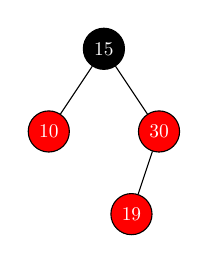
\begin{tikzpicture}[-, level/.style={sibling distance = 2cm/#1, level distance = 1.5cm}, scale=0.7,transform shape]
	\node[circle,draw, fill=black, text=white](z){$15$}
			child{
					node[circle,draw, fill=red, text=white]{10}
			}
			child{
				node[circle,draw, fill=red, text=white]{30}
				child {
					node[circle,draw, fill=red, text=white]{19}
				}
				child[missing]
			};
\end{tikzpicture}
$\Rightarrow$
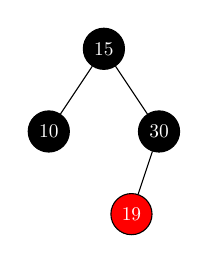
\begin{tikzpicture}[-, level/.style={sibling distance = 2cm/#1, level distance = 1.5cm}, scale=0.7,transform shape]
	\node[circle,draw, fill=black, text=white](z){$15$}
			child{
					node[circle,draw, fill=black, text=white]{10}
			}
			child{
				node[circle,draw, fill=black, text=white]{30}
				child {
					node[circle,draw, fill=red, text=white]{19}
				}
				child[missing]
			};
\end{tikzpicture}
\end{center}

Next, we will insert 22. This will be right below 19. Now we have two red nodes under each other which violates the red-black tree. The new node has a black nil node as uncle, so we will first perform a left-rotate on the subtree of 19. This brings 19 left below 22. Now 19 is a left child, we will recolor 22 to black, 30 to red and perform a right-rotation on the subtree of 30.
\begin{center}
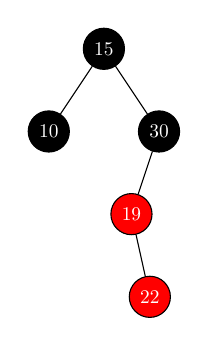
\begin{tikzpicture}[-, level/.style={sibling distance = 2cm/#1, level distance = 1.5cm}, scale=0.7,transform shape]
	\node[circle,draw, fill=black, text=white](z){$15$}
			child{
					node[circle,draw, fill=black, text=white]{10}
			}
			child{
				node[circle,draw, fill=black, text=white]{30}
				child {
					node[circle,draw, fill=red, text=white]{19}
					child[missing]
					child{
						node[circle,draw, fill=red, text=white]{22}
					}
				}
				child[missing]
			};
\end{tikzpicture}
$\Rightarrow$
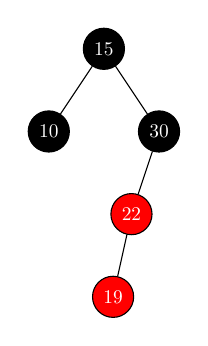
\begin{tikzpicture}[-, level/.style={sibling distance = 2cm/#1, level distance = 1.5cm}, scale=0.7,transform shape]
	\node[circle,draw, fill=black, text=white](z){$15$}
			child{
					node[circle,draw, fill=black, text=white]{10}
			}
			child{
				node[circle,draw, fill=black, text=white]{30}
				child {
					node[circle,draw, fill=red, text=white]{22}
					child{
						node[circle,draw, fill=red, text=white]{19}
					}
					child[missing]
				}
				child[missing]
			};
\end{tikzpicture}
$\Rightarrow$
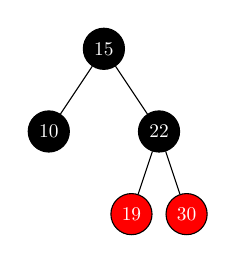
\begin{tikzpicture}[-, level/.style={sibling distance = 2cm/#1, level distance = 1.5cm}, scale=0.7,transform shape]
	\node[circle,draw, fill=black, text=white](z){$15$}
			child{
					node[circle,draw, fill=black, text=white]{10}
			}
			child{
				node[circle,draw, fill=black, text=white]{22}
				child {
					node[circle,draw, fill=red, text=white]{19}
				}
				child {
					node[circle,draw, fill=red, text=white]{30}
				}
			};
\end{tikzpicture}
\end{center}

Finally, we insert 50. This node will be right below 30. Because 50 has a red uncle, we will recolor the nodes 19, 30 and 22 to restore the properties of the red-black tree.
\begin{center}
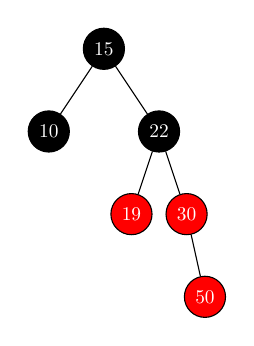
\begin{tikzpicture}[-, level/.style={sibling distance = 2cm/#1, level distance = 1.5cm}, scale=0.7,transform shape]
	\node[circle,draw, fill=black, text=white](z){$15$}
			child{
					node[circle,draw, fill=black, text=white]{10}
			}
			child{
				node[circle,draw, fill=black, text=white]{22}
				child {
					node[circle,draw, fill=red, text=white]{19}
				}
				child {
					node[circle,draw, fill=red, text=white]{30}
					child[missing]
					child{
						node[circle,draw, fill=red, text=white]{50}
					}
				}
			};
\end{tikzpicture}
$\Rightarrow$
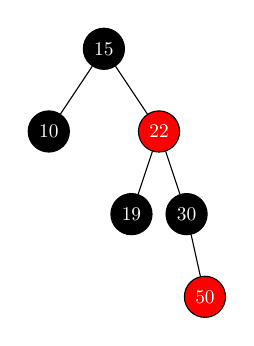
\begin{tikzpicture}[-, level/.style={sibling distance = 2cm/#1, level distance = 1.5cm}, scale=0.7,transform shape]
	\node[circle,draw, fill=black, text=white](z){$15$}
			child{
					node[circle,draw, fill=black, text=white]{10}
			}
			child{
				node[circle,draw, fill=red, text=white]{22}
				child {
					node[circle,draw, fill=black, text=white]{19}
				}
				child {
					node[circle,draw, fill=black, text=white]{30}
					child[missing]
					child{
						node[circle,draw, fill=red, text=white]{50}
					}
				}
			};
\end{tikzpicture}
\end{center}

The first node we will delete is 10. This unbalances the tree since the black height of the root is 1 on the left side and two on the right side. The black nil node that comes on the position of 10 has a red sibling. This means we can perform a left-rotation. After this rotation we need to recolor 22 to black, since it's the new root. We should also recolor 19, to keep the black height of the root balanced.
\begin{center}
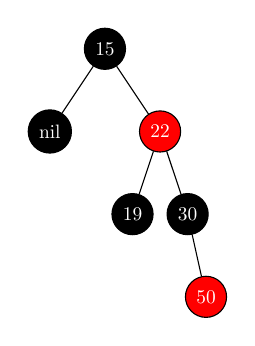
\begin{tikzpicture}[-, level/.style={sibling distance = 2cm/#1, level distance = 1.5cm}, scale=0.7,transform shape]
	\node[circle,draw, fill=black, text=white](z){$15$}
			child{
					node[circle,draw, fill=black, text=white]{nil}
			}
			child{
				node[circle,draw, fill=red, text=white]{22}
				child {
					node[circle,draw, fill=black, text=white]{19}
				}
				child {
					node[circle,draw, fill=black, text=white]{30}
					child[missing]
					child{
						node[circle,draw, fill=red, text=white]{50}
					}
				}
			};
\end{tikzpicture}
$\Rightarrow$
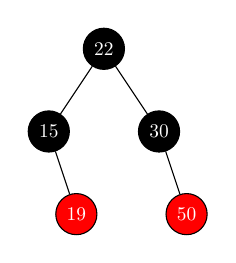
\begin{tikzpicture}[-, level/.style={sibling distance = 2cm/#1, level distance = 1.5cm}, scale=0.7,transform shape]
	\node[circle,draw, fill=black, text=white](z){$22$}
			child{
					node[circle,draw, fill=black, text=white]{15}
					child[missing]
					child {
						node[circle,draw, fill=red, text=white]{19}
					}
			}
			child{
				node[circle,draw, fill=black, text=white]{30}
				child[missing]
				child {
					node[circle,draw, fill=red, text=white]{50}
				}
			};
\end{tikzpicture}
\end{center}

The last deletion we perform will be the deletion of 30. In this deletion 50 will become a child of 22. Since 50 has a black sibling, we will recolor 50 to black to balance the black heigth of the root.
\begin{center}
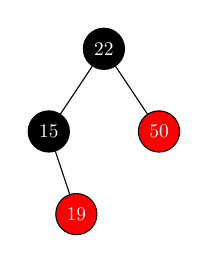
\begin{tikzpicture}[-, level/.style={sibling distance = 2cm/#1, level distance = 1.5cm}, scale=0.7,transform shape]
	\node[circle,draw, fill=black, text=white](z){$22$}
			child{
					node[circle,draw, fill=black, text=white]{15}
					child[missing]
					child {
						node[circle,draw, fill=red, text=white]{19}
					}
			}
			child{
				node[circle,draw, fill=red, text=white]{50}
			};
\end{tikzpicture}
$\Rightarrow$
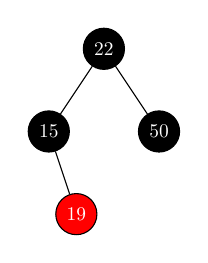
\begin{tikzpicture}[-, level/.style={sibling distance = 2cm/#1, level distance = 1.5cm}, scale=0.7,transform shape]
	\node[circle,draw, fill=black, text=white](z){$22$}
			child{
					node[circle,draw, fill=black, text=white]{15}
					child[missing]
					child {
						node[circle,draw, fill=red, text=white]{19}
					}
			}
			child{
				node[circle,draw, fill=black, text=white]{50}
			};
\end{tikzpicture}
\end{center}

\newpage
\subsection*{Exercise 3. \textit{Weight: 20\%}}
In this exercise, we focus on the insertion of elements in a RBT.
\begin{enumerate}
	\item What do we need to do when the RBT contained no element before insertion?
	\item What do we need to do when the parent of the inserted node $N$ is black?
	\item Suppose here that the parent of $N$, $P$ is red. Show that $N$ has a grand-parent $G$ who is black, and has an uncle $U$.
	\item In case $U$ is black, show that you can reestablish the properties of a RBT by at most 2 rotations and 2 nodes re-coloring.
	\item Last case: $U$ is red. Note here that $P$ violates condition "If a node is red, then both its children are black". What can we do if $G$ is the root of the RBT?
\end{enumerate}

\subsection*{Solutions 3}
\begin{enumerate}
	\item Insert a red node as root in the tree. We should immediately recolor this node to black to fulfill the red-black tree properties.
	\item We may insert a red node.
	\item Since P is red, we know that it isn't the root of the tree, since the root needs to be black. This means that the grandparent can be the root or another black node. The grandparent has to be black when it's not the root, because if it would be red, then P had to be black to fulfill the red-black tree properties before insertion. We know that there is a uncle, because whether a black nil node will be the uncle or there will be another node as uncle.
	\item In case that there is an uncle, we know that there a parent and grandparent should exist. These should already fulfill the properties of a red-black tree before this insertion. We know that the grandparent and uncle are black and the parent is red. So after the insertion of N, the red parent P has a red child which violates the properties of a red black tree. Since N has a black uncle, we should recolor P to black and G to red. We also should perform a left-rotate to re-establish the properties of a red-black tree. A visual representation of this action is shown in figure~\ref{Fig:M1}.
\begin{figure}[h]
\begin{center}
	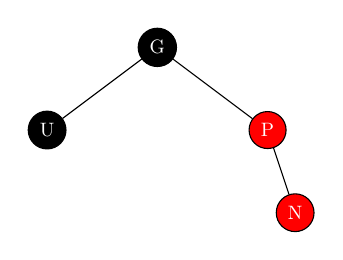
\begin{tikzpicture}[-, level/.style={sibling distance = 2cm/#1, level distance = 1.5cm}, scale=0.7,transform shape]
		\node[circle,draw, fill=black, text=white](z){G}
				child{
						node[circle,draw, fill=black, text=white]{U}
				}
				child[missing]
				child {
					node[circle,draw, fill=red, text=white]{P}
					child[missing]
					child{
						node[circle,draw, fill=red, text=white]{N}
					}
				};
	\end{tikzpicture}
	$\Rightarrow$
	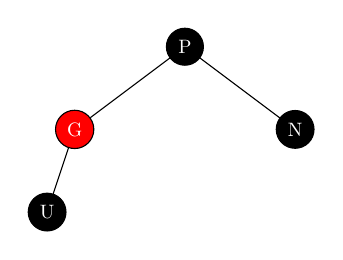
\begin{tikzpicture}[-, level/.style={sibling distance = 2cm/#1, level distance = 1.5cm}, scale=0.7,transform shape]
		\node[circle,draw, fill=black, text=white](z){P}
				child{
						node[circle,draw, fill=red, text=white]{G}
						child{
							node[circle,draw, fill=black, text=white]{U}
						}
						child[missing]
				}
				child[missing]
				child {
					node[circle,draw, fill=black, text=white]{N}
				};
	\end{tikzpicture}
	\caption{Tree with black uncle} \label{Fig:M1}
	\end{center}
\end{figure}
At the end we recolored two nodes, namely P and G. Furthermore, we only did perform one rotation. So, we indeed recolored at most two nodes and had even less than two rotations.
	\item Since N has a red uncle, we should recolor the parent, uncle and grandparent. This means the parent and uncle will become black and the grandparent red. But since G is the root of the tree, we should recolor it to a black node to fulfill the red-black tree properties. This means that afterwards only the parent and uncle are recolored to black.
\end{enumerate}

\newpage
\section*{Part II. Revisions.}

\subsection*{Exercise 4. \textit{Weight: 20\%}}
Suppose a CS curriculum consists of $n$ courses, all of them mandatory.
The prerequisite graph $G$ has a node for each course, and an edge from course $v$ to course $w$ if and only if $v$ is a prerequisite for $w$. Find an algorithm that works directly with this graph representation, and computes the minimum number of semesters necessary to complete the curriculum (assume that a student can take any number of courses in one semester). The running time of your algorithm should be linear.

\subsection*{Solutions 4}
In order to find the minimum amount of semesters, we should find the longest path from the source, since two courses for which holds that one course is a prerequisite for the other cannot be followed at the same time. Courses that have no relation may be followed simultaneously. This means the number of edges in the longest possible path is the number of minimum semesters. A possible graph representation is drawn in figure~\ref{Fig:M2}.

In order to find the longest path we can make use of a modified DFS which also stores the distance from the source. DFS has a linear complexity and is able to find paths. DFS originally only stores the discovery time and finishing time. In this version we should also add a parameter for the lenth of the path from the first node like BFS has. We should also make sure that DFS starts at the beginning of each path when there are still undiscovered edges.

Another modification we should make is that when a node is already finished and it has a shorter distance than the new path + 1, then we should visit it and modify the distance value to path + 1. This may only happen when the new path using the discovered node is longer.
After running DFS all nodes are having the length from the first cource assigned. These distances are shown above the nodes in figure~\ref{Fig:M2}.

In the example we can see that the highest distance is 4, since the first node has distance 0 we will add 1 to it to get the length of the path. In the algorithm we can iterate through the list of nodes and find the maximum distance value and return this incremented with 1 as the minimum amount of semesters necessary to complete the curriculum. This iteration trough all vertices will also be performed linear.

So, the solution is a DFS based on BFS. BFS isn't suitable since the algorithm would only find one path.

\begin{figure}[h]
	\begin{center}
		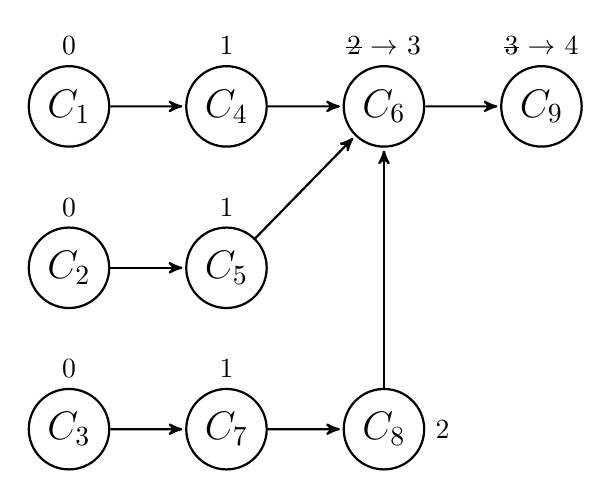
\begin{tikzpicture}[->,>=stealth',shorten >=1pt,auto,node distance=2cm, every loop/.style={},
		                    thick, ,main node/.style={circle,draw,font=\sffamily\Large\bfseries}, scale=0.7]

		  % \node[main node] (1) [label=0] {s};
		  \node[main node] (3) [label=0] {$C_2$};
			\node[main node] (2) [above=1cm and 3cm of 3, label=0] {$C_1$};
		  \node[main node] (4) [below=1cm and 3cm of 3, label=0] {$C_3$};
		  \node[main node] (5) [right of=2, label=1] {$C_4$};
			\node[main node] (6) [right of=3, label=1] {$C_5$};
			\node[main node] (7) [right of=5, label=\sout{2} $\rightarrow$ 3] {$C_6$};
			\node[main node] (8) [right of=4, label=1] {$C_7$};
			\node[main node] (9) [right of=8, label={[align=center]right:2}] {$C_8$};
			\node[main node] (10) [right of=7, label=\sout{3} $\rightarrow$ 4] {$C_9$};

		  \path[every node/.style={font=\sffamily\normalsize, text = black }]
		    % (1) edge[black] node [below] {} (2)
				% 		edge[black] node [below] {} (3)
				% 		edge[black] node [below] {} (4)
				(2)	edge[black] node [below] {} (5)
				(3)	edge[black] node [below] {} (6)
				(4)	edge[black] node [below] {} (8)
				(5) edge[black] node [below] {} (7)
				(6)		edge[black] node [below] {} (7)
				(7) edge[black] node [below] {} (10)
				(8) edge[black] node [below] {} (9)
				(9) edge[black] node [below] {} (7);
		\end{tikzpicture}
	\end{center}
	\caption{Example graph representation} \label{Fig:M2}
\end{figure}

\newpage
\subsection*{Exercise 5. \textit{Weight: 20\%}}
There is a network of roads $G = (V, E)$ connecting a set of cities $V$.
Each road in $E$ has an associated length.
There is a proposal to add one new road to this network, and there is a list $E'$ of pairs of cities between which the new
road can be built.
Each such potential road $e \in E'$ has an associated length $l_e$.
As a designer for the public works department you are asked to determine the road in $E'$ whose addition to the existing network $G$
would result in the maximum decrease in the driving distance between two fixed cities $s$ and $t$ in the network.
Give an efficient algorithm for solving this problem.

\subsection*{Solutions 5}
 An undirected graph with roads as edges between the cities. We can try for each road in E' to add it to the graph and find out which road gives the shortest length between s and t. The shortest length between s and t is equal to the path with the maximum decrease between s and t, since the maximum decrease of the length will lead to a path that's shorter than the other possible paths. After each possible edge we should check whether the length of the path decreased and if so we should save it.

 In order to calculate the shortest path between s and t we may use the Dijkstra algorithm. We should perform this algorithm for every potential road in E'. After we executed this for every $e \in E'$, we should return the shortest path when there exists a shorter path in the potential roads.

 Dijkstra has a complexity of $O(|E|lg|V|)$, so performing Dijkstra for every edge in E' will cost $O(|E'||E|lg|V|)$ in total. This solution isn't that very efficient, but could solve the problem.

\newpage
\subsection*{Exercise 6. \textit{Weight: 20\%}}
A directed graph is \emph{semiconnected} if, for all pairs of vertices $u$, $v$, there is either a path from $u$ to $v$,
or there is a path from $v$ to $u$.
Give an efficient algorithm to determine whether or not a directed graph is semiconnected.
Prove that you algorithm is correct and analyze its running time.

\subsection*{Solutions 6\footnote{Made use of the following video for clarification about the problem: \href{https://www.youtube.com/watch?v=2E7tzF4ihvI}{https://www.youtube.com/watch?v=2E7tzF4ihvI}}.}
There may exist two types of graphs for this problem. The graph may be circular or it could be a directed acyclic graph. In the case of a circular graph it's clear that it's semiconnected, since we may take each path also in the other direction in the cycle.

In the case that it's a DAG we may perform a topological sort on the graph. This sort uses DFS to first discover the deepest edges. After an edge is finished it's placed in the stack. After this, the stack contains all nodes in the order in which they may be reached. We should convert this stack in a list with the same order. In a semiconnected graph this order will always be the same. If the graph is semiconnected there should be a path to all other vertices from the vertex that's on top of the stack.

An example of a graph that is semiconnected can be found in figure~\ref{Fig:M3}. When we run this algorithm on this graph a possible stack is shown in table~\ref{Table:T1}. We see that E is on top of the stack and that ther is a path possible from E to all other nodes.

An example of a graph that is not semiconnected can be found in figure~\ref{Fig:M4}. We see in this example that there is no path $A \to E$ in one of the directions possible which makes it not semiconnected. In this stack A is on top. However, there is no path possible from A to E. This shows the graph is not semiconnected.

To analyze whether we may reach all other vertices from the top node of the stack, we could perform BFS with the topnode as source and check for all distances in the nodes whether they are known.

The topological sort on the graph has a complexity of $O(|V| + |E|)$. The BFS that is executed after this has a linear complexity of $O(|V| + |E|)$. The check whether all nodes are reached from the top node has a complexity of $O(V)$. This brings the complexity of the total algorithm to $O(|V| + |E|)$ which is linear.

\begin{figure}[h]
	\begin{center}
	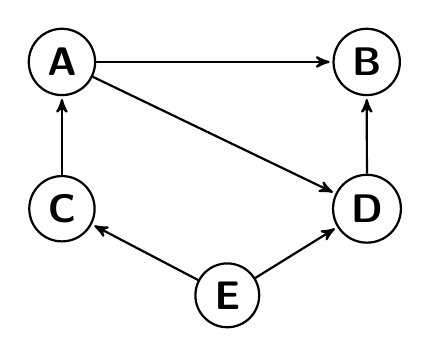
\begin{tikzpicture}[->,>=stealth',shorten >=1pt,auto,node distance=2cm, every loop/.style={},
	                    thick, ,main node/.style={circle,draw,font=\sffamily\Large\bfseries}]

	  \node[main node] (1) {A};
	  \node[main node] (2) [right=1cm and 3cm of 1] {B};
	  \node[main node] (3) [below=1cm and 2cm of 1] {C};
	  \node[main node] (4) [right=1cm and 3cm of 3] {D};
	  \node[main node] (5) [below right=0.5cm and 1.5cm of 3] {E};

	  \path[every node/.style={font=\sffamily\normalsize, text = black }]
	    (1) edge[black] node [below] {} (2)
					edge[black] node [below] {} (4)
			(3)	edge[black] node [below] {} (1)
			(4)	edge[black] node [below] {} (2)
			(5) edge[black] node [below] {} (3)
					edge[black] node [below] {} (4);
	\end{tikzpicture}
	\caption{A semiconnected graph} \label{Fig:M3}
	\end{center}
\end{figure}
\begin{table}
	\begin{center}
	\begin{tabular}{c | c}
	Finished   & Discovered	\\ \hline
	E           & E         \\
	C           & B       	\\
	A           & D       	\\
	D           & A      		\\
	B           & C       	\\
	\end{tabular}
	\end{center}
	\caption{Stack for graph in figure~\ref{Fig:M3}} \label{Table:T1}
\end{table}

\begin{figure}[h]
	\begin{center}
	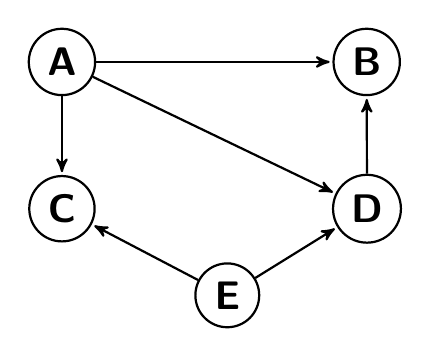
\begin{tikzpicture}[->,>=stealth',shorten >=1pt,auto,node distance=2cm, every loop/.style={},
											thick, ,main node/.style={circle,draw,font=\sffamily\Large\bfseries}]

		\node[main node] (1) {A};
		\node[main node] (2) [right=1cm and 3cm of 1] {B};
		\node[main node] (3) [below=1cm and 2cm of 1] {C};
		\node[main node] (4) [right=1cm and 3cm of 3] {D};
		\node[main node] (5) [below right=0.5cm and 1.5cm of 3] {E};

		\path[every node/.style={font=\sffamily\normalsize, text = black }]
			(1) edge[black] node [below] {} (2)
					edge[black] node [below] {} (3)
					edge[black] node [below] {} (4)
			(4)	edge[black] node [below] {} (2)
			(5) edge[black] node [below] {} (3)
					edge[black] node [below] {} (4);
	\end{tikzpicture}
\end{center}
	\caption{Not a semiconnected graph} \label{Fig:M4}
\end{figure}
\begin{table}
	\begin{center}
	\begin{tabular}{c | c}
	Finished   & Discovered	\\ \hline
	A           & A         \\
	E           & B       	\\
	D           & D       	\\
	B           & E      		\\
	C           & C       	\\
	\end{tabular}
	\end{center}
	\caption{Stack for graph in figure~\ref{Fig:M4}} \label{Table:T2}
\end{table}

\end{document}
